%!TEX root = report.tex
\newcommand{\R}{\mathbb{R}}
\section{Methodology}
\label{Sec:methodology}

%Methodology/Algorithm: What method or algorithm are you proposing? If there are existing implementations, will you use them and how? How do you plan to improve or modify such implementations?

Our project will start from the state-of-the-art convolutional neural network model. Sentence word embeddings are concatenated together as inputs, $(h_1,h_2,\ldots,h_n)$, where the maximum sentence length are $n$ words. If a sentence is less than $n$ words, we will use zero word vectors to fill it. Therefore, our input data are consistent length $n$. Next, a convolutional layer is performed on the sentence word embeddings with a width-two window to $d$-channel filters of size $n-1$. Then a max pooling layer pick the largest value among the $n-1$ layers and form a $d$-channel features. Finally, this length $d$ features are input into a softmax layer to classify three-class label. In mathematical equation:
\begin{equation}
	\mathbf{c_i} = \tanh(W_L\mathbf{h_i} + W_R \mathbf{h_{i+1}} + \mathbf{b}), i=1,2,\ldots,n-1
\end{equation}
where $\mathbf{h_i}\in \R^{D\times1}$ are word embedding, $\mathbf{c_i} \in \R^{d\times1}$ are padding $i$ in the convolutional layer, $W_L$ and $W_R$ are convolutional layer kernel matrices, $\mathbf{b}$ is the convolutional layer bias vector.
\begin{equation}
	\mathbf{s} = \max_{i=1,2,\ldots,n-1}\mathbf{c_i}
\end{equation}
where $\mathbf{s} \in \R^{d \times 1}$ are features learned from CNN.
\begin{equation}
	\mathbb{P}(Y=c|s)=\frac{\exp(W_{c}\mathbf{s}+\mathbf{b_c})}{\sum_{c'}\exp(W_{c'}\mathbf{s}+\mathbf{b_c'})}
\end{equation}


\begin{figure}[htbp] %  figure placement: here, top, bottom, or page
   \centering
   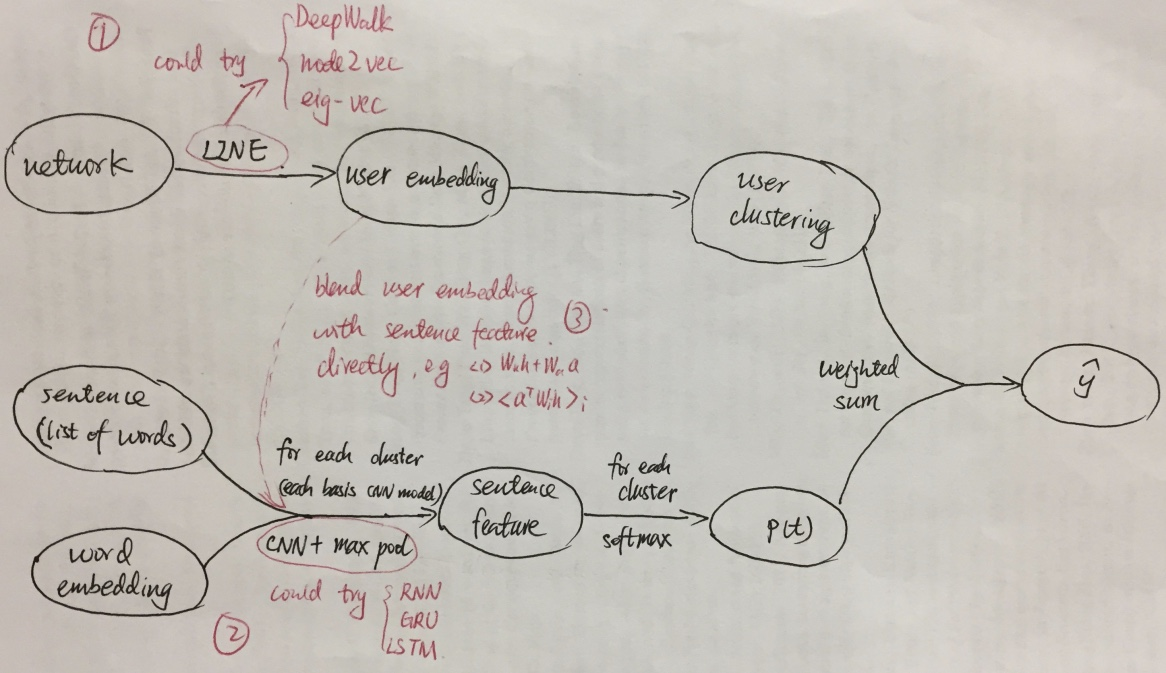
\includegraphics[width=5.2in]{flow.jpg} 
   \caption{General Methodology}
   \label{Fig:Flow}
\end{figure}



We are going to extend this model in three aspects, as is illustrated in the red lines in Figure \ref{Fig:Flow}. To be specific, 
\begin{enumerate}   [(1)]
%\setcounter{enumi}{3}
\item Using other node embedding methods in network analysis, such as \textit{DeepWalk}[2] and \textit{node2vec}[3];
\item Explore other methods to combine author information and sentence information, especially the bilinear form $a^T W h$ which measures the interaction between author and sentence. Here $a$ is the author embedding and $h$ is the sentence embedding.
\item Explore other models in sentiment analysis, such as RNN, GRU, and LSTM.
\end{enumerate}
